\documentclass{article}
\usepackage{dsfont}
\usepackage{graphicx}
\usepackage{amsfonts,amssymb}
\usepackage{amsmath}
\usepackage{fancyhdr}
\usepackage{enumerate}
\usepackage{hyperref}
\usepackage{bm}
\usepackage{xcolor}
\usepackage{graphicx}
\usepackage{geometry}
\usepackage{stmaryrd}
\usepackage{multirow}
\usepackage{booktabs}
\usepackage{float}
\usepackage{subfig}
\usepackage{physics}
\usepackage{fancyvrb}
\geometry{top=0.5cm,bottom=0.5cm}
\usepackage[section]{placeins}
\title{Unsupervised learning using clustering--- Mining the 20 Newsgroups Dataset}
\author{Haining Pan}
\begin{document}
    \maketitle
    \section{Introduction}
    In this report, we study the similarity of newsgroups by utilizing several unsupervised learning clustering algorithms, including `Kmeans', `Agglomerative clustering', and `DBSCAN'.
    The newsgroups are composed of text files, such as posts, messages, and emails. 
    We use the built-in dataset `fetch\_20newsgroups' in `Sklearn'.~\cite{20newsgroups}
    The dataset carries the labels, therefore, our ultimate goal here is to see how well we can reproduce the given label using unsupervised learning clustering. This project is inspired by and generalized on ~\cite{book}.
    \section{Dataset}
    The 20 newsgroups dataset contains around 18000 posts on 20 topics. In this project, we choose 4 topics, 'rec.sport.baseball','talk.politics.guns','comp.graphics','sci.med' , which contains 3867 posts (samples).

    \subsection{Preprocessing}
    \subsection{Bag of word}
    We use the bag-of-word (BoW) model, which converts a text into a vector by counting the frequency of each word. Therefore, the number of features is just the number of different words in the whole dataset.

    However, there are some words does not carry too much information, such as the name, numbers, and stop words. Therefore, we also remove them by using `NLTK' package. 

    Furthermore, to account for the variant morphosis of the same word (e.g., `sit' and `sitting', `desk' and `desks'), we `lemmatize' words in order to create redundant features by using `WordNetLemmatizer' in `NLTK'.

    \subsection{TF-IDF}

    Before we feed our vectors of term frequency into the clustering algorithms, we address the issue of the information that each word carries, because the more common a word appears in the whole sample, the less distinct information it carries. This is implemented by using the term frequency-inverse document frequency (TF-IDF). Therefore, the final data we feed into the clustering algorithms is the sparse matrix of the size of (n\_samples, n\_features) after the data preprocessing, where we name it `data' in the code. 


    \section{Clustering}
    In this section, we perform the clustering on the sparse matrix of `data'. To save the pages, we directly show results, while the code is provided in the GitHub repository.~\cite{Github}
    \subsection{Kmeans}
    We start with the Kmeans, and sweep the number of clusters, as shown in Fig.~\ref{fig:kmeans}, where we use Silhouette score and inertia as the metrics to evaluate the clustering results.

    
    \begin{figure}[ht]
        \centering
        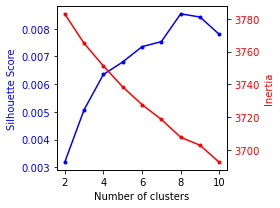
\includegraphics[width=.5\textwidth]{kmeans}
        \caption{Silhouette score (left axis) and inertia (right axis) as a function of the number of clusters in Kmeans.}
        \label{fig:kmeans}
    \end{figure}

    In Fig.~\ref{fig:kmeans}, we notice the number of clusters $k=4$ seems to be an inflection point in Elbow Method, while $k=8$ gives the largest Sihouette score. Therefore, we treat these two ($k=4$ and $k=8$) as candidates, which will be later used to compare with the original labels by calculating the Rand Index.


    \subsection{Agglomerative clustering}
    We next apply the agglomerative clustering as shown in Fig.~\ref{fig:Agg}. 
    
    \begin{figure}[ht]
        \centering
        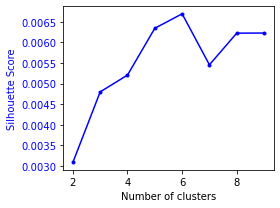
\includegraphics[width=.5\textwidth]{Agg}
        \caption{Silhouette score as a function of the number of clusters in Agglomerative clustering}
        \label{fig:Agg}
    \end{figure}

    In Fig.~\ref{fig:Agg}, we notice that $k=6$ has the highest Silhouette score, while $k=5$ is roughly the same. Therefore, we save these two estimators which are later used to compare with the original labels. 

    \subsection{DBSCAN}
    Finally, we apply the DBSCAN and use `GridSearchCV' to find the best $\epsilon$ and `min\_samples'. We vary $\epsilon$ between 0.5 and 1.5 in a step of 0.1, and `min\_samples' between 2 and 15, and calculate the corresponding Silhouette score, as shown in Fig.~\ref{fig:dbscan}.

    
    \begin{figure}[ht]
        \centering
        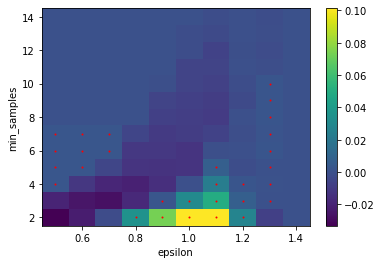
\includegraphics[width=.5\textwidth]{DBSCAN}
        \caption{Silhouette score as a function of $\epsilon$ and `min\_samples'. The red dots mark the parameters with positive Silhouette scores.}
        \label{fig:dbscan}
    \end{figure}

    In Fig.~\ref{fig:dbscan}, we find most of the parameters give negative Silhouette scores, and only a few specific points give positive Silhouette scores, which are marked in red. Therefore, we will focus on these red dots, and see whether they can provide us with meaningful clusters in the next step.

    We apply the DBSCAN again with parameters shown in red dots in Fig.~\ref{fig:dbscan}. The results are shown in Table~\ref{tab}. 

    \begin{table}[h]
        \caption{Silhouette score and the number of clusters for the DBSCAN model with different parameters of $\epsilon$ and `num\_samples'.}
        \label{tab}
        \begin{tabular}{|l|l|l|l|l|l|l|l|l|l|l|l|l|l|l|l|l|l|l|l|l|l|l|l|l|l|l|l|l}
        \hline
        ($\epsilon$ ,num\_samples) &(0.5, 4)& (0.5, 5)& (0.5, 6)& (0.5, 7)& (0.6, 5)& (0.6, 6)& (0.6, 7)& (0.7, 6)\\
        \hline
        Silhouette score & 0.0028&0.0028&0.0028&0.0028&0.0028&0.0028&0.0028&0.0028 \\
        \hline
        Num\_clusters & 2&2&2&2&2&2&2&2\\        
        \hline
        \hline
        ($\epsilon$ ,num\_samples) & (0.7, 7)& (0.8, 2) & (0.9, 2)& (0.9, 3)& (1, 2)& (1, 3)& (1.1, 2)& (1.1, 3) \\
        \hline
        Silhouette score & 0.0028&0.0346&0.0731&0.0028&0.1008&0.0307&0.1013&0.0498\\
        \hline
        Num\_clusters & 2&423&564&175&651&273&619&314\\
        \hline
        \hline
        ($\epsilon$ ,num\_samples) & (1.1, 4)& (1.1, 5)& (1.2, 2)& (1.2, 3)& (1.2, 4)& (1.3, 3) & (1.3, 4) & (1.3, 5)\\
        \hline        
        Silhouette score & 0.0235&0.0070&0.0274&0.0071&0.0023&0.0004&0.0007&0.0003\\
        \hline
        Num\_clusters & 181&102&334&150&104&5&4&3 \\
        \hline
        \hline
        ($\epsilon$ ,num\_samples) & (1.3, 6)& (1.3, 7)& (1.3, 8)& (1.3, 9)& (1.3, 10) &&&\\
        \hline
        Silhouette score &  0.0020&0.0020&0.0020&0.0020&0.0020 &&&\\
        \hline
        Num\_clusters & 2&2&2&2&2 &&&\\
        \hline
        \end{tabular}
        
        \end{table}

        From Table~\ref{tab}, we notice that 1) most of the models have either just two clusters or unreasonably many clusters, which are not meaningful. Therefore, we doubt the applicability of DBSCAN here, since the original data may be highly inhomogeneous in the density. Nevertheless, we still choose models with 4, 5, and 6 clusters above, and see what the clusters are in those models.

    \section{Final evaluation}

    Finally, we use the adjusted Rand Index to test the clustering from the different models above. For Kmeans, we obtain 0.5 for $k=4$ and 0.34 for $k=8$. For agglomerative clustering, we obtain  0.6 for $k=5$ and 0.59 for $k=6$. For DBSCAN, we obtain all very small values of Rand Index: 0.00026 for (1.3, 3), 0.00038 for (1.3, 4), and 0.00072 for (1.3,5). 

    To show explicitly what each cluster contains, we print 1. the size of each cluster; 2. the size of original labels that each cluster contains; 3. Top 10 words in each cluster. 

    For kmeans with $k=4$, we have 
    \begin{Verbatim}
cluster_0: 698 samples
Top Keywords: gun/wa/people/fbi/government/article/atf/right/law/batf
	talk.politics.guns: 697 samples
	sci.med: 1 samples
cluster_1: 751 samples
Top Keywords: game/team/wa/player/baseball/article/hit/win/pitcher/brave
	rec.sport.baseball: 750 samples
	talk.politics.guns: 1 samples
cluster_2: 670 samples
Top Keywords: graphic/image/file/program/format/need/university/looking/know/bit
	comp.graphics: 660 samples
	sci.med: 8 samples
	rec.sport.baseball: 2 samples
cluster_3: 1748 samples
Top Keywords: wa/article/university/ha/know/like/just/doe/medical/computer
	sci.med: 981 samples
	comp.graphics: 313 samples
	rec.sport.baseball: 242 samples
	talk.politics.guns: 212 samples
    \end{Verbatim}

    For kmeans with $k=8$, we have
    \begin{Verbatim}
cluster_0: 382 samples
Top Keywords: wa/fbi/atf/batf/government/waco/burn/dividian/article/people
	talk.politics.guns: 381 samples
	sci.med: 1 samples
cluster_1: 706 samples
Top Keywords: game/team/wa/player/baseball/hit/article/pitcher/brave/win
	rec.sport.baseball: 705 samples
	sci.med: 1 samples
cluster_2: 1435 samples
Top Keywords: university/wa/article/know/doe/just/ha/like/thanks/computer
	comp.graphics: 537 samples
	sci.med: 402 samples
	rec.sport.baseball: 289 samples
	talk.politics.guns: 207 samples
cluster_3: 317 samples
Top Keywords: gun/people/firearm/right/law/weapon/wa/like/article/criminal
	talk.politics.guns: 317 samples
cluster_4: 439 samples
Top Keywords: image/graphic/file/program/format/bit/color/need/computer/display
	comp.graphics: 435 samples
	sci.med: 4 samples
cluster_5: 58 samples
Top Keywords: msg/food/sensitivity/chinese/restaurant/reaction/eat/allergic/people/effect
	sci.med: 58 samples
cluster_6: 455 samples
Top Keywords: doctor/ha/wa/medical/patient/disease/pain/yeast/article/drug
	sci.med: 449 samples
	talk.politics.guns: 5 samples
	comp.graphics: 1 samples
cluster_7: 75 samples
Top Keywords: shameful/chastity/surrender/gordon/bank/pittsburgh/science/computer/article/lyme
	sci.med: 75 samples

    \end{Verbatim}


    For agglomerative clustering with 5 clusters, we have
    \begin{Verbatim}
cluster_0: 839 samples
Top Keywords: game/wa/team/player/baseball/article/hit/ha/win/think
	rec.sport.baseball: 815 samples
	sci.med: 13 samples
	comp.graphics: 6 samples
	talk.politics.guns: 5 samples
cluster_1: 791 samples
Top Keywords: gun/wa/people/fbi/article/government/right/atf/like/law
	talk.politics.guns: 772 samples
	comp.graphics: 9 samples
	sci.med: 6 samples
	rec.sport.baseball: 4 samples
cluster_2: 1416 samples
Top Keywords: wa/article/university/ha/know/medical/science/like/doe/computer
	sci.med: 896 samples
	comp.graphics: 227 samples
	rec.sport.baseball: 166 samples
	talk.politics.guns: 127 samples
cluster_3: 58 samples
Top Keywords: msg/food/sensitivity/chinese/restaurant/allergic/eat/reaction/people/flavor
	sci.med: 58 samples
cluster_4: 763 samples
Top Keywords: graphic/image/file/program/university/need/format/computer/know/bit
	comp.graphics: 731 samples
	sci.med: 17 samples
	rec.sport.baseball: 9 samples
	talk.politics.guns: 6 samples
    \end{Verbatim}

    For agglomerative clustering with 6 clusters, we have 
    \begin{Verbatim}
cluster_0: 791 samples
Top Keywords: gun/wa/people/fbi/article/government/right/atf/like/law
	talk.politics.guns: 772 samples
	comp.graphics: 9 samples
	sci.med: 6 samples
	rec.sport.baseball: 4 samples
cluster_1: 763 samples
Top Keywords: graphic/image/file/program/university/need/format/computer/know/bit
	comp.graphics: 731 samples
	sci.med: 17 samples
	rec.sport.baseball: 9 samples
	talk.politics.guns: 6 samples
cluster_2: 1416 samples
Top Keywords: wa/article/university/ha/know/medical/science/like/doe/computer
	sci.med: 896 samples
	comp.graphics: 227 samples
	rec.sport.baseball: 166 samples
	talk.politics.guns: 127 samples
cluster_3: 58 samples
Top Keywords: msg/food/sensitivity/chinese/restaurant/allergic/eat/reaction/people/flavor
	sci.med: 58 samples
cluster_4: 803 samples
Top Keywords: game/team/wa/player/article/hit/baseball/ha/win/brave
	rec.sport.baseball: 779 samples
	sci.med: 13 samples
	comp.graphics: 6 samples
	talk.politics.guns: 5 samples
cluster_5: 36 samples
Top Keywords: jewish/baseball/come/hank/sandy/racking/lame/john/wa/article
	rec.sport.baseball: 36 samples

    \end{Verbatim}

    For DBSCAN with (1.3,3), we have 
    \begin{Verbatim}
cluster_0: 3754 samples
Top Keywords: wa/ha/world/like/university/heard/research/article/similar/japanese
	rec.sport.baseball: 984 samples
	comp.graphics: 953 samples
	sci.med: 930 samples
	talk.politics.guns: 887 samples
cluster_1: 4 samples
Top Keywords: wa/article/university/ha/like/know/just/think/people/gun
	sci.med: 4 samples
cluster_2: 5 samples
Top Keywords: leung/drink/ng/ho/lactose/intolerance/experiencing/milk/ton/hardly
	sci.med: 5 samples
cluster_3: 3 samples
Top Keywords: centipede/millipede/posionous/pes/bitten/liable/clarification/know/concerted/soon
	comp.graphics: 3 samples
cluster_4: 3 samples
Top Keywords: playmation/retail/ren/hitchhiking/kenbaer/anjon/hash/sell/scn/marino
	sci.med: 3 samples
    \end{Verbatim}

    For DBSCAN with (1.3,4), we have
    \begin{Verbatim}
cluster_0: 3725 samples
Top Keywords: wa/ha/world/like/university/article/research/playmation/know/information
	rec.sport.baseball: 979 samples
	comp.graphics: 948 samples
	sci.med: 918 samples
	talk.politics.guns: 880 samples
cluster_1: 4 samples
Top Keywords: wa/article/university/ha/like/know/just/think/people/gun
	sci.med: 4 samples
cluster_2: 4 samples
Top Keywords: leung/drink/ng/ho/lactose/intolerance/experiencing/milk/ton/hardly
	sci.med: 4 samples
cluster_3: 5 samples
Top Keywords: acne/oily/face/teenage/skin/wash/son/clearasil/dalacin/nose
	sci.med: 5 samples
    \end{Verbatim}

    For DBSCAN with (1.3,5), we have
    \begin{Verbatim}
        cluster_0: 3698 samples
        Top Keywords: wa/ha/university/article/world/like/information/think/know/leung
            rec.sport.baseball: 976 samples
            comp.graphics: 945 samples
            sci.med: 902 samples
            talk.politics.guns: 875 samples
        cluster_1: 5 samples
        Top Keywords: wa/article/university/ha/like/know/just/think/people/gun
            sci.med: 5 samples
        cluster_2: 4 samples
        Top Keywords: centipede/millipede/posionous/pes/bitten/liable/clarification/know/concerted/soon
            sci.med: 4 samples        
    \end{Verbatim}
    





    
    
    \section{Conclusion}

    In summary, the best performance of clustering is reached by agglomerative clustering with the Rand Index of $\sim$ 0.6. The explicit number of clusters does not matter that much between 5 and 6, as they bascially refer to the same types of clustering. For the 6 clusters, there are two clusters (cluster3 and cluster5) that are not well distinguished, however, these two clusters have very small sizes, which can be reasonably ignored. Besides that, agglomerative clustering identifies most clusters correctly. 

    For kmeans, the best model is the one with 4 clusters although the model with 8 clusters has a larger Silhouette score. However, it is generally worse than agglomerative clustering, as it always leaves a cluster containing all four original labels, which indicates there are some texts that kmeans cannot distinguish. (For example, cluster3 in k=4) However, besides that cluster, all other three clusters are classified quite well, which is as good as the agglomerative method.

    For DBSCAN, it cannot produce meaningful clusters, as it simply classifies all samples into one big cluster (which is the boundary with label -1 by further check) 
    This could be due to the intrinsic inhomogeneous density in the dataset, therefore, DBSCAN is not very useful in such a text-based situation.

    \section{Reference}

    \begin{thebibliography}{9}
        \bibitem{20newsgroups}
        \hyperref{https://scikit-learn.org/stable/datasets/real\_world.html\#newsgroups-dataset}{}{}{https://scikit-learn.org/stable/datasets/real\_world.html\#newsgroups-dataset}
        \bibitem{book}
        Chapter 3, Python Machine Learning By Example, Liu Yuxi, PacktPub
        \bibitem{Github}
        \hyperref{https://github.com/hainingpan/UnsupervisedLearning/blob/master/UL.ipynb}{}{}{https://github.com/hainingpan/UnsupervisedLearning/blob/master/UL.ipynb}

    \end{thebibliography}





\end{document}